In our experiments, we sought to find and compare four different aspects of the 
file system in a host OS running natively on a machine and in a guest OS running
on top of the host. We found and compared the ideal buffer size for random file 
access, prefetch size, file cache size, and at what sizes the file system adds 
another layer of inode pointers in the following subsections.

\subsection{Ideal Buffer Size for Random I/O}
\label{sec:p1}
The first parameter we measured was the ideal buffer size for random I/O 
on a file. First, let us define what we mean by "ideal buffer size." Since
the time to read data is affected by the amount of data read, we define ideal
buffer size as the size in which we achieve the best throughput (Bytes/s)
with the smallest amount of memory. 

Given the classical formula of Equation~\ref{eq:p1_latency} for the latency 
of a magnetic disk access:

\begin{equation}\label{eq:p1_latency}
Latency = S + R + DataSize/TransferRate + C
\end{equation}

where S = Seek Time, R = Rotational Delay, and C = Controller delay, we 
derive the throughput as $T = \frac{DataSize}{Latency}$. We assume that S, R, 
and C are roughly constant regardless of size, so we represent them as constant K and simplify to Equation~\ref{eq:p1_throughput}:

\begin{equation}\label{eq:p1_throughput}
T = \frac{DataSize}{K + \frac{DataSize}{TransferRate}}
\end{equation}

We expect the throughput to follow the behavior of a rational function
with an asymptote equalling TransferRate as DataSize becomes infinitely large.
Thus, the ideal buffer size is defined as the minimum DataSize for which the 
throughput is equal to the TransferRate. In the virtual machine case, we assume 
that the overhead due to address translation is marginal due to the shadow page 
tables, so we expect the VM throughput to be approximately the same as in the host.

In order to measure the throughput, we used the test described by the pseudocode 
of Figure~\ref{fig:p1code}. We first measured the latency to read a
certain number of bytes from disk. Then we calculated throughput T by dividing 
readSize by the latency. However, there were a few aspects we needed 
to consider in our experiment. Since prefetch occurs on sequential read, 
we avoided the problem of measuring the time to retrieve data from the cache instead
of disk access time by first reading a single byte from the end of the file
and then reading from a random offset, essentially making the Linux readahead
algorithm interpret both reads as random. Moreover, we flushed the cache in
between each change of the readSize. 

\begin{figure}[h!]
\begin{lstlisting}
for readSize := MAX_READ_SIZE to MIN_READ_SIZE do
   clear cache
   open file
   read 1B from the end of the file
   t1 := rdtsc_start()
   read readSize bytes from random offset 
   t2 := rdtsc_end()
   close file
\end{lstlisting} 
\caption{Pseudocode for measuring ideal buffer size}
\label{fig:p1code}
\end{figure}

%% Graphs, Results
\begin{figure}[ht!]
	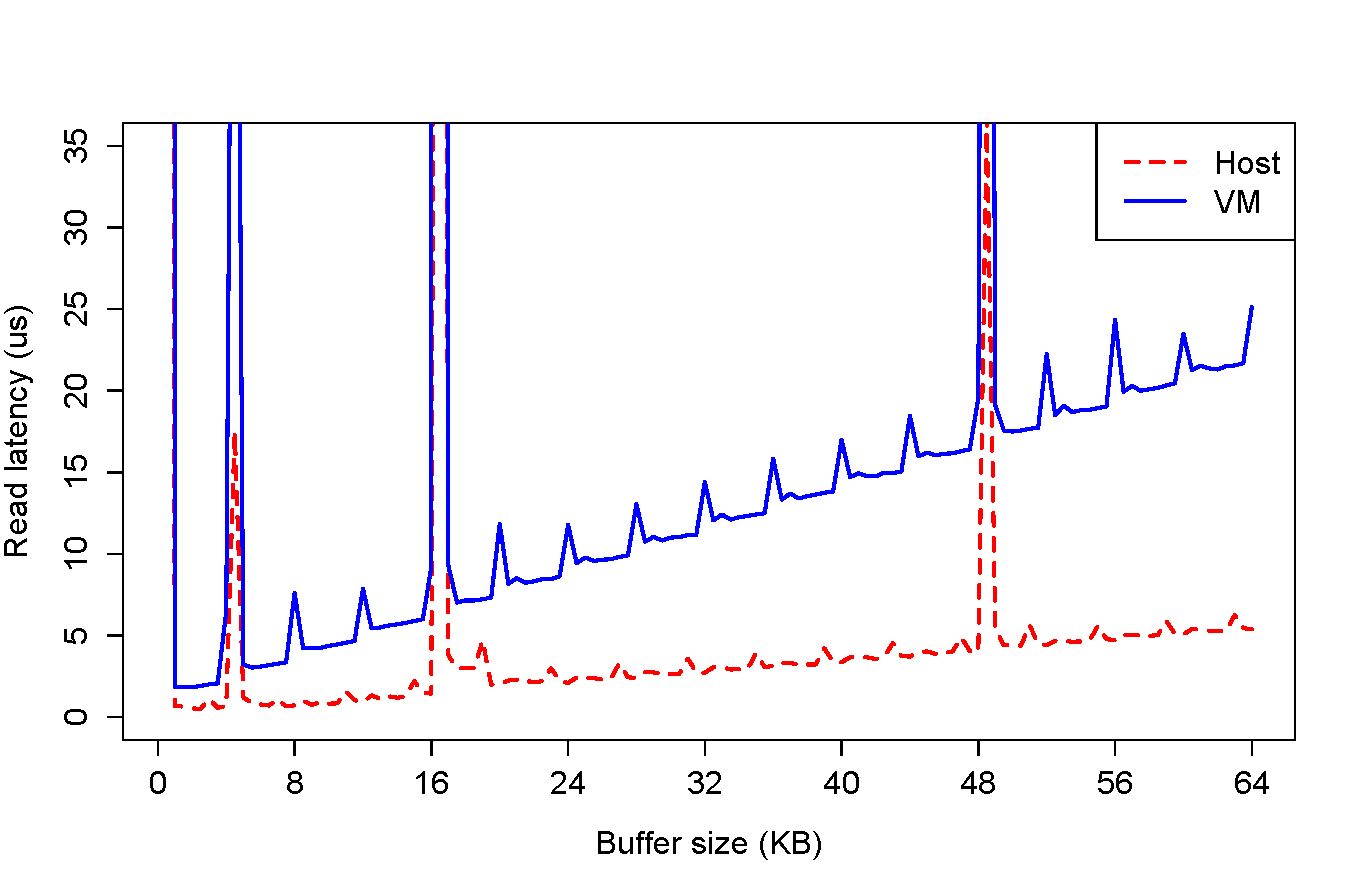
\includegraphics[width=0.5\textwidth]{./figures/p1.pdf}
	\caption{}
	\label{fig:p1graph}
\end{figure}




\subsection{Prefetch Size}
\label{sec:p2}
We were able to measure the prefetch size read by the system during a sequential 
read. In Linux, there is a readahead algorithm that fetches a certain number of 
pages from disk given the read behavior. The set of pages in the cache fetched by 
the algorithm is called the readahead window. In a normal sequential read, the 
readahead algorithm starts with an initial read size based on the first read and in
subsequent requests grows the readahead window until it reaches the maximum size. 
The readahead algorithm marks a page at the lookahead index. When the application 
references this page, the algorithm grows the readahead window and asynchronously 
fetches the next set of pages from disk. The maximum window is determined by 
parameters in the kernel code, but it is typically 32 pages. In our system, we have
4KB pages so we expect the readahead size to grow exponentially and then plateau at
the maximum window size of 128KB. We expect the same for our virtual machine, which 
has the same readahead algorithm and page size.

\begin{figure}[t!]
	\begin{algorithmic}
		\STATE open $file$
		\STATE flush cache
		\FOR{$i = $0 \TO $MAX\_READS$}
		\STATE start\_timer
		\STATE Read READ\_SIZE bytes
		\STATE end\_timer and save the result
		\STATE Wait 100ms
		\ENDFOR
		\STATE close $file$
		\STATE report recorded times
	\end{algorithmic}
	\caption{Pseudocode for measuring prefetch size}
	\label{fig:p2_code}
\end{figure}

\begin{figure}[hb!]
	\begin{subfigure}[t]{0.5\textwidth}
	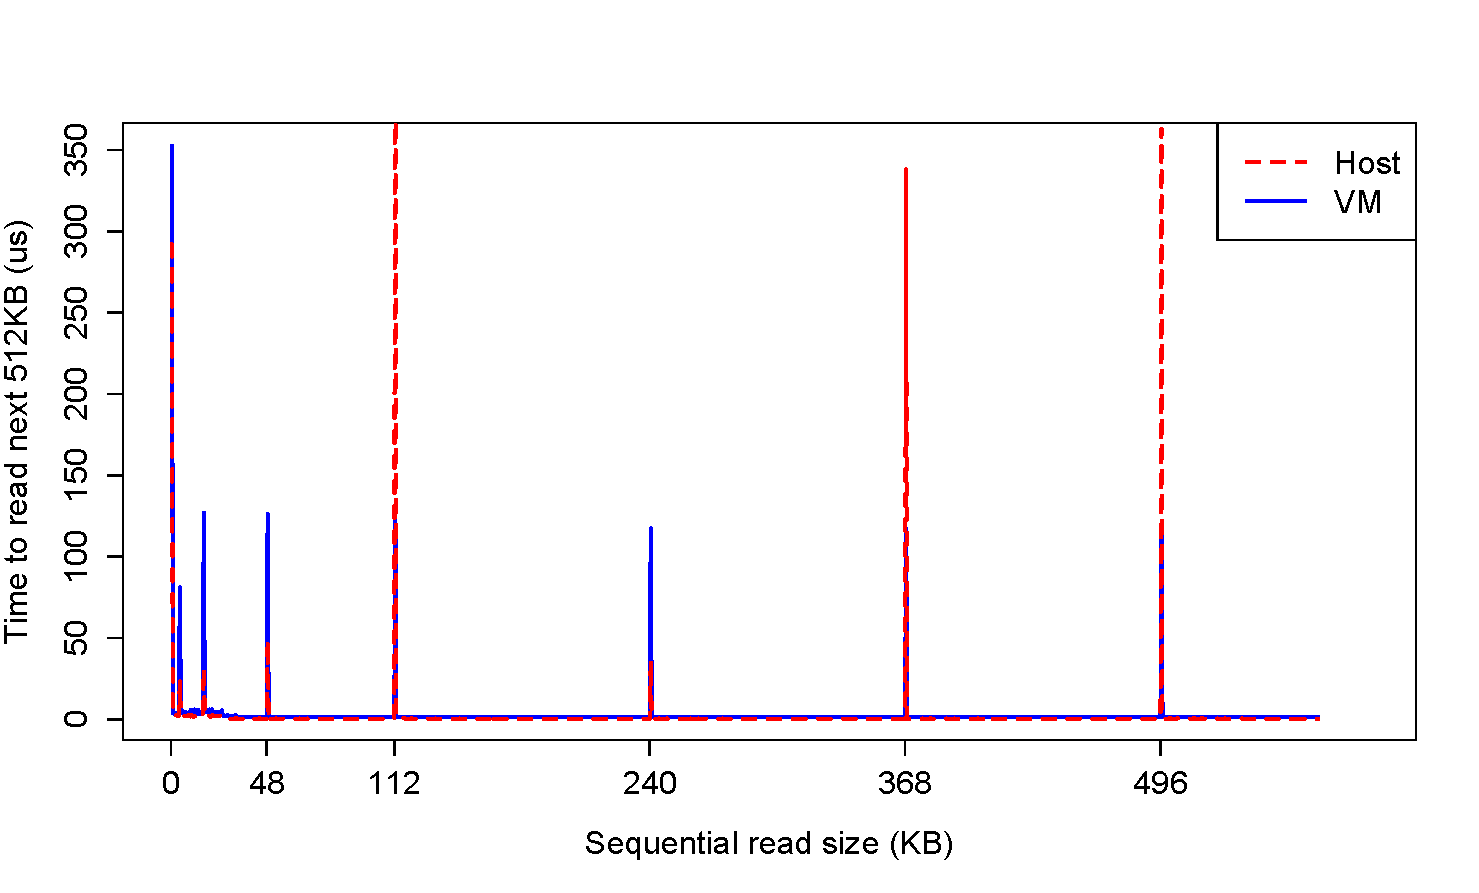
\includegraphics[width=\textwidth]{./figures/p2_big.pdf}
	\caption{A broad view of latency versus number of read bytes}
	\label{fig:p2_graph_big}
	\end{subfigure}
	
	\begin{subfigure}[t]{0.5\textwidth}
	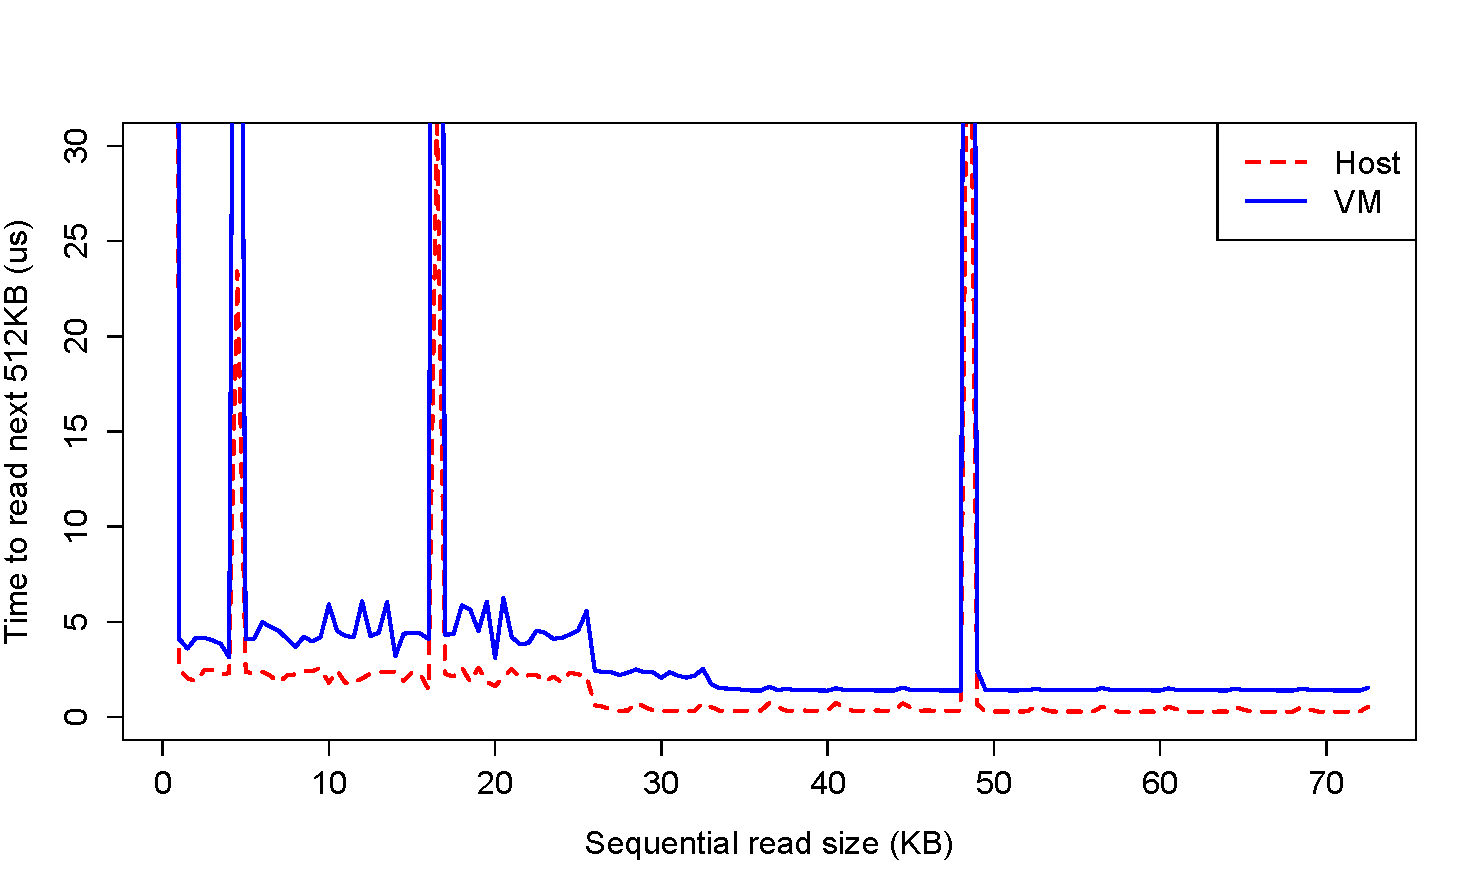
\includegraphics[width=\textwidth]{./figures/p2_small.pdf}
	\caption{A close up view of latency versus number of read bytes}
	\label{fig:p2_graph_small}
	\end{subfigure}
	\caption{Time to read 512KB blocks with respect to total number of KB read sequentially from a file}
\end{figure}

Since the read latency is much greater when the requested page is not in the page 
cache, we can find the prefetch size by performing sequential reads and determining
the sizes in which spikes occur. We assume that the lookahead index is the last 
page of the readahead window. With this in mind, we wrote the code of 
Figure~\ref{fig:p2_code} to measure the prefetch size. In our code, we flush 
the cache before the initial read and measure the time to read READ\_SIZE number of
bytes at a time. We then wait 100ms to allow time for pages to be prefetched. This
eliminates false positives in the case where the read requests occur faster than
the data can be fetched from disk, resulting in a page fault.

Figure~\ref{fig:p2_graph_big} shows the read latency for a READ\_SIZE of 512B with
respect to the total number of bytes read. We see spikes for the host and VM at the same
places in the read sequence. We observe high latency for the initial read, and
then at increasing intervals of 4KB, 12KB, 32KB, and 64KB. After this the spikes occur
at fixed intervals of 128KB. Thus, readahead behaves as we expect with an window that
grows until it reaches the maximum prefetch size.






\subsection{File Cache Size}
\label{sec:p3}
Next, we measured the file cache size. Our hypothesis is that file cache size is dynamic and that it depends on the amount of free memory available to the system since it would not make sense for the system to keep a lot of free pages around when it could use them to speed up sequential reads.

To check our hypothesis, we designed two controlled experiments with different amounts of free memory available to the system. One experiment runs with most of the memory unused. In the other experiment, we allocate a huge array and fill it with random data to avoid page sharing effects. We call this array \emph{balloon}. We used a 10GB balloon in the host environment and a 3GB balloon in the virtual machine since they had different RAM sizes.

Each experiment consists of four repeated sequential reads of varying size. We measure throughput on last three reads. If the read size is smaller than the file cache size, the data accessed in repeated reads reside in the cache, making repeated reads very fast. As soon as the size of our reads exceeds the cache size, we expect to see huge decrease in total throughput since some of the repeated reads will need to go to disk and wait for I/O. Figure \ref{fig:p3pseudo} shows the pseudocode of the experiments. We used 20MB for the buffer size, guided by insight from Section \ref{sec:p1}. In the virtual environment we had to be careful to avoid the effects of the host file cache so we flushed the host file cache before every read.

\begin{figure}
\begin{algorithmic}
\STATE clear cache
\IF {ballooning enabled}
\STATE allocate huge array
\STATE fill the array with random data
\ENDIF
\STATE $size \leftarrow$ {sequential read size}
\STATE $file \leftarrow$ {huge file filled with random data}
\STATE $buffer\_size \leftarrow$ 20MB
\STATE flush the cache
\STATE read first $size$ bytes of $file$
\FOR{$i = 0$ to $3$}
\IF {running in VM}
\STATE clear host file cache
\ENDIF
\STATE open $file$
\WHILE{total bytes read $< size$}
\STATE start\_timer
\STATE read next $buffer\_size$ bytes
\STATE end\_timer and save the result
\ENDWHILE
\STATE close $file$
\ENDFOR
\STATE report average of all timers divided by $buffer\_size$
\end{algorithmic}
\caption{Function used to measure file cache size}
\label{fig:p3pseudo}
\end{figure}

Figure \ref{fig:p3graph} shows the repeated read throughput for each measured sequential read size. We observe the expected behavior for all four cases. First, we see a sharp decrease in throughput after a certain point: 6GB for VM with ballooning, 8GB for the VM without ballooning, 12GB for the host with ballooning, and 22GB for the host without ballooning. We attribute this effect to read sizes getting bigger than the file cache. Next, we observe a smaller file cache size when running experiments with ballooning, which proves our hypothesis that the file cache size is dynamic and depends on the amount of free memory available to the system. The difference between the points of sharp decline in throughput for the cases with and without ballooning -- 2GB for the VM and 10GB for the host -- is roughly the size of the balloon. We attribut the disparity for the VM case due to the granularity of our measurement, which rounds down to the nearest GB. It is interesting to note that the kernel did not decide to swap out the balloon array and increase the file cache size, even though it would speed up execution of our program. However, we can not make any inferences about the general policy of swapping out memory to increase file cache size. (TODO maybe phrase this better)

\begin{figure}[ht!]
	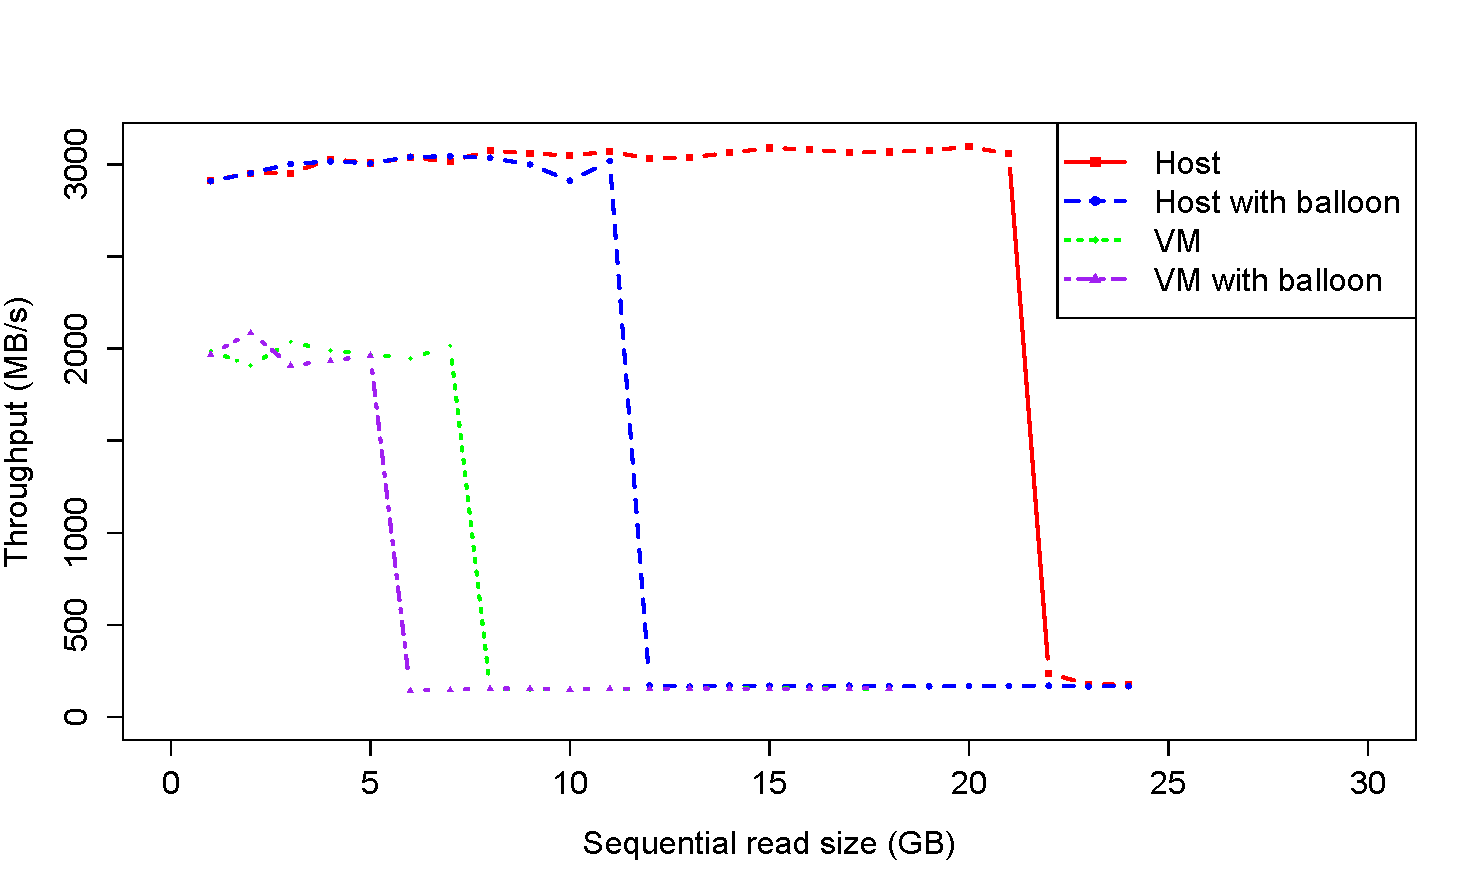
\includegraphics[width=0.5\textwidth]{./figures/p3.pdf}
	\caption{Repeated sequential read throughput. Horizontal axis shows size of repeated sequential read and vertical axis shows throughput. Throughput was measured in four environments: Host with a lot of free memory, Host with 10GB balloon, Virtual Machine with a lot of free memory and Virtual Machine with 3GB balloon.}
	\label{fig:p3graph}
\end{figure}


\subsection{Inode Pointer Indirection}
\label{sec:p4}
Our final goal was to determine file sizes for which file system adds another layer of indirection. Ext4 uses extents to manage data blocks. \cite{ext4extents} Extents are organized into a tree, where each extent can point either to another extent (interior extent) or to a block group (leaf extent). A block group is a physically continuous range of blocks, where each block is 4096 bytes. Each block group can address up to $2^{15}$ continuous blocks, which is total of 128 MB. Each inode stores direct pointers to up to four leaf extents. When the file size outgrows the four existing extents and the filesystem creates a fifth extent, it also creates a new metadata block. At that point, we say that the filesystem adds one layer of indirection.


Let us consider three scenarios that might happen when we append one block to the file:
\begin{enumerate}
\item \textbf{The last block group in the file is extended.} In this case, the file system writes a data block and updates one block group.
\item \textbf{There is no more space left in the last block group.} The file system needs to create a new block group and a new extent.
\item \textbf{There is no more space left in the last block group, and all four extents in the file inode are used.} The file system needs to create a new block group, a new extent, and also reorganize the four extents in the file inode.
\end{enumerate}

The assumption we need to make to be able to detect these events is that case 3 is considerably slower than 2 and that case 2 is considerably slower than 1. We also need to assume that any other slowdown that might happen during the process of writing bytes is uncorrelated with the file size and will be eliminated by only taking into account the lower bound of multiple runs.

\begin{figure}[t!]
\begin{algorithmic}
\STATE create a $file$
\STATE $buffer\_size \leftarrow$ 4096
\FOR{$i = 0$ to $MAX\_SIZE$}
\STATE $buffer \leftarrow$ random $buffer\_size$ bytes
\STATE open a file with O\_SYNC flag, seek to the end
\STATE start\_timer
\STATE write first byte of $buffer$
\STATE end\_timer and save the result
\STATE write the rest $buffer\_size - 1$ bytes
\STATE close a file
\ENDFOR
\end{algorithmic}
\caption{Function used to measure one-byte append latency}
\label{fig:p4pseudo}
\end{figure}

Group blocks in ext4 can be arbitrarily sized and depend on disk layout. If a block following the group block is used, the file system needs to create a new group block. If it is free, the file system just extends the group block. Because of this, we hypothesize that the moment when ext4 adds another layer of indirection does not depend only on file size but also on the disk layout and other factors.

We propose the experiment presented in Figure \ref{fig:p4pseudo} to verify our hypothesis. By timing a one-byte append, we should be able to distinguish between when the file system creates a new extent (cases 2 and 3) and a normal append (case 1). We run the experiment five times and take the minimum latency for each data point. If our hypothesis holds and adding a layer of indirection does not depend solely on file size, we expect to see a flat line as a result of our experiment. This result would also confirm our expectation that there is no single file size in which an append would cause spikes in latency due to creating new metadata blocks.

\begin{figure}[t!]
    \begin{subfigure}[b]{0.5\textwidth}
		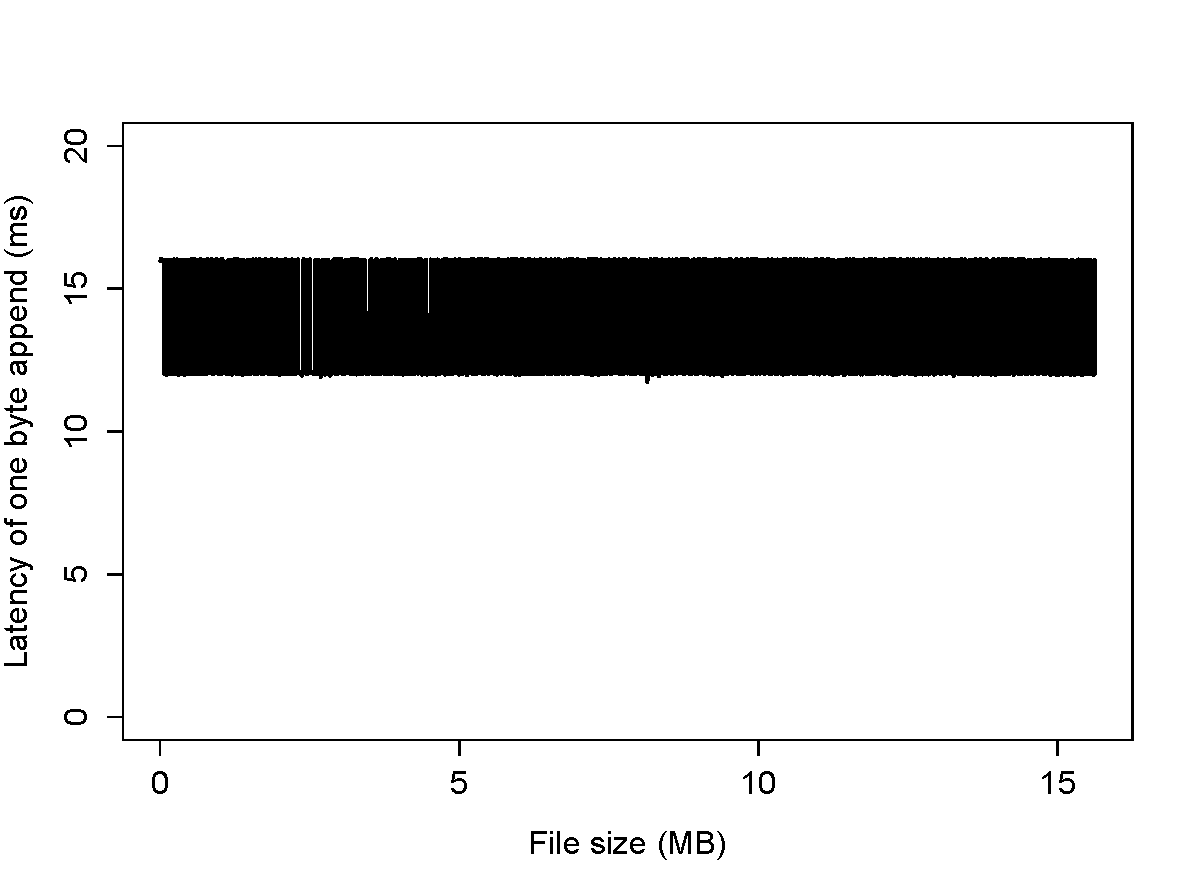
\includegraphics[width=1\textwidth]{./figures/p4_host.pdf}
		\caption{Host}
		\label{fig:p4host}
    \end{subfigure}
    \begin{subfigure}[b]{0.5\textwidth}
		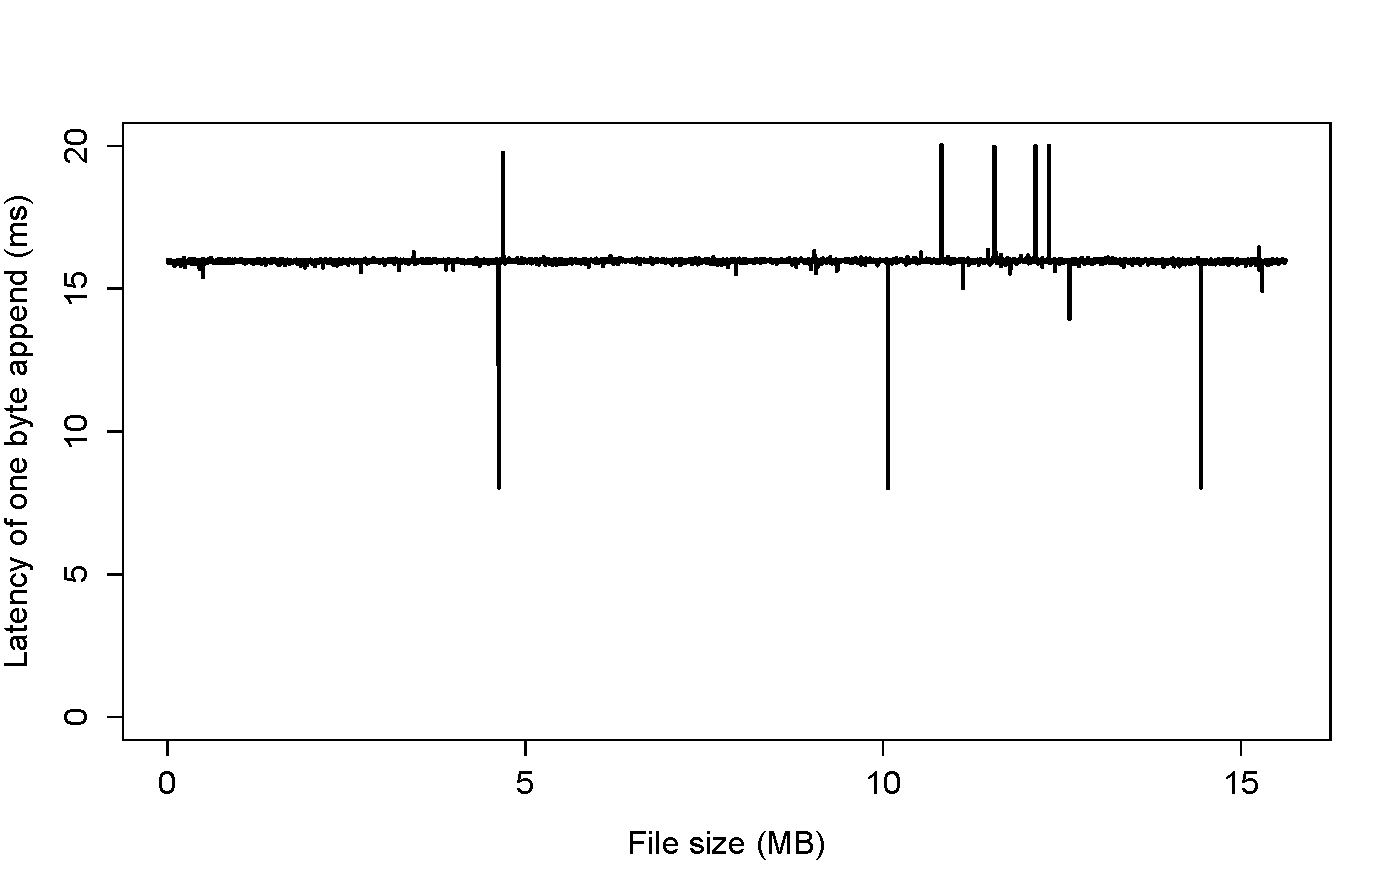
\includegraphics[width=1\textwidth]{./figures/p4_vm.pdf}
		\caption{Virtual machine}
		\label{fig:p4vm}
    \end{subfigure}
	\caption{Latency of one-byte append for varying file sizes. Horizontal axis shows existing file size and vertical axis shows latency of appending one byte to that file.}
	\label{fig:p4}
\end{figure}


Figure \ref{fig:p4} shows the measured latency of a one-byte append to files of variable sizes. Every data point is the minimum latency that we obtained over five experiment runs. In the host, each write took either 12 or 16ms. Results in the host environment clearly show that we could not identify any file size for which we would see a consistently slower append operation. We did, however, observe large write latency spikes in individual test runs. We also confirmed that some of the resulting files indeed had an extent tree with an indirection layer by using \texttt{debugs} to examine file extent tree.

Given that our assumptions hold, these results prove our hypothesis that the moment when indirection layer is inserted does not depend only on file size in ext4.

In the virtual machine, most of the writes take 16ms. However, we observe spikes at 4804KB, 11076KB, 11832KB, 11844KB, 12420KB and 12612KB. We also see unusually fast latencies for some writes. These spikes might possibly be results of building indirection layers at those specific file sizes. However, they might also be results of other anomalies in the virtualized environment. We did not further investigate those issues. Our results from running experiments in the virtual machine neither prove nor refute the hypothesis.



